\documentclass[conference]{IEEEtran}

\usepackage{url}
\usepackage{amsmath}
\usepackage{graphicx}
\usepackage{subfigure}

\begin{document}


\author{
\IEEEauthorblockN{Dimitris Mitropoulos\IEEEauthorrefmark{1}, Vassilios Karakoidas\IEEEauthorrefmark{1},
Georgios Gousios\IEEEauthorrefmark{2}, Panagiotis Louridas\IEEEauthorrefmark{1},
Diomidis Spinellis\IEEEauthorrefmark{1}}\\
\IEEEauthorblockA{\IEEEauthorrefmark{1}Department of Management Science and Technology\\
Athens University of Economics and Business\\
\{dimitro, bkarak, louridas, dds\}@aueb.gr}\\
\IEEEauthorblockA{\IEEEauthorrefmark{2}TODO: Add Affiliation here\\
Delft University of Technology\\
G.Gousios@tudelft.nl}}

\title{Dismal Code: Studying the Evolution of Security Bugs}

\maketitle

\begin{abstract}
%\boldmath
Security bugs are critical programming errors that can lead to serious
vulnerabilities in software. Such bugs may allow an attacker to take over
an application, steal data or prevent the application from working at all.
In this paper, we present how we used the Maven repository to study the
characteristics of security bugs individually and in relation to other software
bugs. In particular, we analyzed every project version of the repository by using a
popular static analysis tool. Then by taking advantage of the various features of
the repository (multiple versions for every project, dependencies and others) we studied
the evolution of security bugs through time, their persistence and their relationship with a) the
size of the corresponding version and b) other bug categories. Also, based on the
dependencies of artifacts we constructed the graph of the repository and
examined the most popular nodes based on their PageRank. 
\end{abstract}

\begin{IEEEkeywords}
Software Bugs, Static Analysis, Software Evolution, Software
Security, Maven, FindBugs.
\end{IEEEkeywords}

\IEEEpeerreviewmaketitle

\section{Introduction}

A security bug is a programming error that introduces a potentially
exploitable weakness into a computer system~\cite{SSL12, TJBD11}. This weakness could lead to a
security breach with unfortunate consequences in different layers, like databases,
native code, applications, libraries and others. Despite the significant
effort to detect and eliminate such bugs~\cite{SZ12}, little attention has been paid to
study them in relation to software evolution~\cite{L96, LRWPT97, IB06, RGMA06}.
In this paper we present how we used a large software ecosystem to analyze
how evolving software packages are related to the different types of security
vulnerabilities.

One of the most common approaches to identify security bugs is
{\it static analysis}~\cite{CW07}. This kind of analysis involves the
inspection of the program's source or object code without executing
it. For our research we used {\it FindBugs},\footnote{\url{http://findbugs.sourceforge.net/}}
a static analysis tool that examines bytecode to detect software bugs and has already been used in
research~\cite{AP10, HP07, HP04}. Specifically, we ran FindBugs on all the project
versions of all the projects that exist in the Maven\footnote{\url{http://maven.apache.org/}}
repository (approximately 265GB of data). Then we observed the changes that
involved the security bugs and their characteristics. This research builds upon
our earlier work on the topic~\cite{MGS12}.

We chose to focus our study on the security bugs rather than other
software bugs. This is because compared to other bug categories,
the category of security bugs has two distinct features: it is critical~\cite{SZ12}
and it costs~\cite{BCL08}. Specifically, a software bug can
lead to a mulfunction of a software artifact that runs under specific
requirements but a security bug can allow a malicious user to alter the execution
of the entire application. In this case, such bugs could span a wide
range of security and privacy issues, like viewing sensitive information, the destruction or
modification of sensitive data, denial of service and others.
Moreover, security bug disclosures lead to a negative and significant change
in market value for a software vendor~\cite{TW07}.
Hence, one of the basic pursuits in every new software release should
be the mitigation of such bugs.

The motivation behind our work was to validate if programmers tend to care for
such high-risk bugs when they release a new version of their software. In
addition, we wanted to investigate other critical features associated with such
vulnerabilities like the persistency of a bug. In essence, to check if specific bugs stay
unresolved for a long time. Also, we wanted to elaborate more on the relation of security
bugs not only with performance bugs (as Zaman et al.~\cite{ZAH11} have already
did) but also with other bug categories. In the same manner, we tried to check
the relation between a version's size and its' security bugs knowing the
that research has been contradictory on the the issue~\cite{BP84, SYTP85,
NBZ06, GKMS00}. Finally, we examined the Maven ecosystem as a whole from a security
perspective. Its structure, gave us the oportunity to see if a project version that is a dependency to
a large number of others contains a high rate of security bugs.
In this case we can strenghten the relationship between Linus' Law and
software security as Meneely et al. have already indicated~\cite{MW10}.

The main contributions of this research are:

\begin{itemize}
	\item The analysis of how security bugs evolve over time. To achieve
this, we inspect every project per version. Our hypothesis is that security
bugs must decrease as a project evolves since they are critical and developers
should eliminate them.
	\item Security bug persistense between versions. We show evidence that
specific bugs are not eliminated between versions.
	\item We show evidence of the relation between security bugs and a project
version's size.  Here, size is defined in terms of bytecode.
	\item The correlation of security bugs with other bug categories. We
show evidence that such bugs are correlated with bugs that have to do with
performance, coding practices and others.
%	\item The relation of software dependencies and security bugs. Our
%hypothesis is that an artifact that is a dependency of many other artifacts
%should have a low rate of security bugs. 
\end{itemize}

In the rest of this paper we
describe the processing of our data and our experiment (Section \ref{sec:meth}),
present and discuss the results we obtained (Section \ref{sec:res}),
outline related work (Section \ref{sec:rel}),
and end up with a conclusion and directions for future work (Section \ref{sec:con}).

\section{Methodology}
\label{sec:meth}

\subsection{Experiment}
\label{sec:exp}

Our experiment goal was to collect the metric results of the FindBugs tool.
The process involved four entities (see Table~\ref{tbl:exp}):
a number of {\it workers}, a {\it task queue}
mechanism,\footnote{\url{http://www.rabbitmq.com/}}
a {\it data repository},\footnote{\url{http://www.mongodb.org/}}
and the {\it code repository}, which in our case it was the public Maven 
repository\footnote{\url{http://mvnrepository.com}}.

\begin{table}
\centering
\caption{Experiment Entities}
\label{tbl:exp}
\begin{tabular}{r r r}
\hline
 & Software Package & version\\
 \hline
Worker & Custom Python Script & 2.7\\
Task Queue & RabbitMQ & 3.0.1 \\
Data Repository & MongoDB & 2.2 \\
Code Repository & Maven Repository & January 2012 \\
\hline
\end{tabular}
\end{table}

First, we scanned the Maven repository for appropriate {\sc jar}s and created a
list that included them. We discuss the {\sc jar} selection process in the next 
section. With the {\sc jar} list at hand, we created a series of processing tasks
and added them to the task queue. Then we executed twenty five (Unix-based)
workers that checked out tasks from the queue, processed the data and stored the
results to the data repository.

A typical processing cycle of a worker included the following steps: after
the worker spawns, it requests a task from the queue. This task contains
the {\sc jar} name, which is typically a project version that is downloaded locally.
First, specific {\sc jar} metadata are calculated and stored. Such metadata include
its size, its dependencies, and a number that represents the chronological order of the
release. This order is derived from an {\sc xml} file that
accompanies every project in the Maven repository called {\it
maven-metadata.xml}. Then FindBugs is executed and its results are also stored
in the data repository. When the task is completed the queue is notified and
the next task is requested.

This process was executed for all the available {\sc jar}s in the task queue.
The experiment was executed five times in order to iron out various bugs in
our scripts and validate the results. 

\subsection{Data Provenance}
\label{sec:data}

\begin{table}
\centering
\caption{Descriptive Statistics Measurements for the Maven Repository}
\label{tbl:repository}
\begin{tabular}{l r}
\hline
Measurement & Value\\
 \hline
Projects & 17,505\\
Versions (total) & 114,399\\
Min & 1\\
Max & 337\\
Mean & 6.54\\
Median & 3\\
Range & 336\\
1$^{st}$ Quartile & 1\\
3$^{rd}$ Quartile & 8\\
\hline
\end{tabular}
\end{table}

The subject of our study was the Maven repository. Before analyzing the data of the
repository we performed a number of functional fits on the data. 

Initially, we obtained a snapshot (January 2012) of the Maven repository and
handled it locally to retreive a list of all the names of the project versions
that existed in it. A project version can be uniquely identified by the triplet:
{\it group id}, {\it artifact id} and {\it version}.
Since FindBugs analyzes applications written in the Java
programming language, and the Maven repository
hosts projects from languages other than Java such as Scala, Groovy,
Clojure etc. we filtered out such projects by performing a series of checks in
the repository data and metadata.

In addition, we implemented a series of audits in the worker scripts that
checked if the {\sc jar}s are valid in terms of implementation. For instance,
for every {\sc jar} the worker checked if there were any {\it .class} files
before invoking FindBugs. After the project filtering we narrowed down
our data set to 17,055 projects with 114,399 versions.
Table~\ref{tbl:repository} summarises the data set information and
provides the basic descriptive statistic measurements. The distribution of version
count among the selected projects is presented in Figure \ref{fig:version-count}.

\begin{figure*}
	\centering
	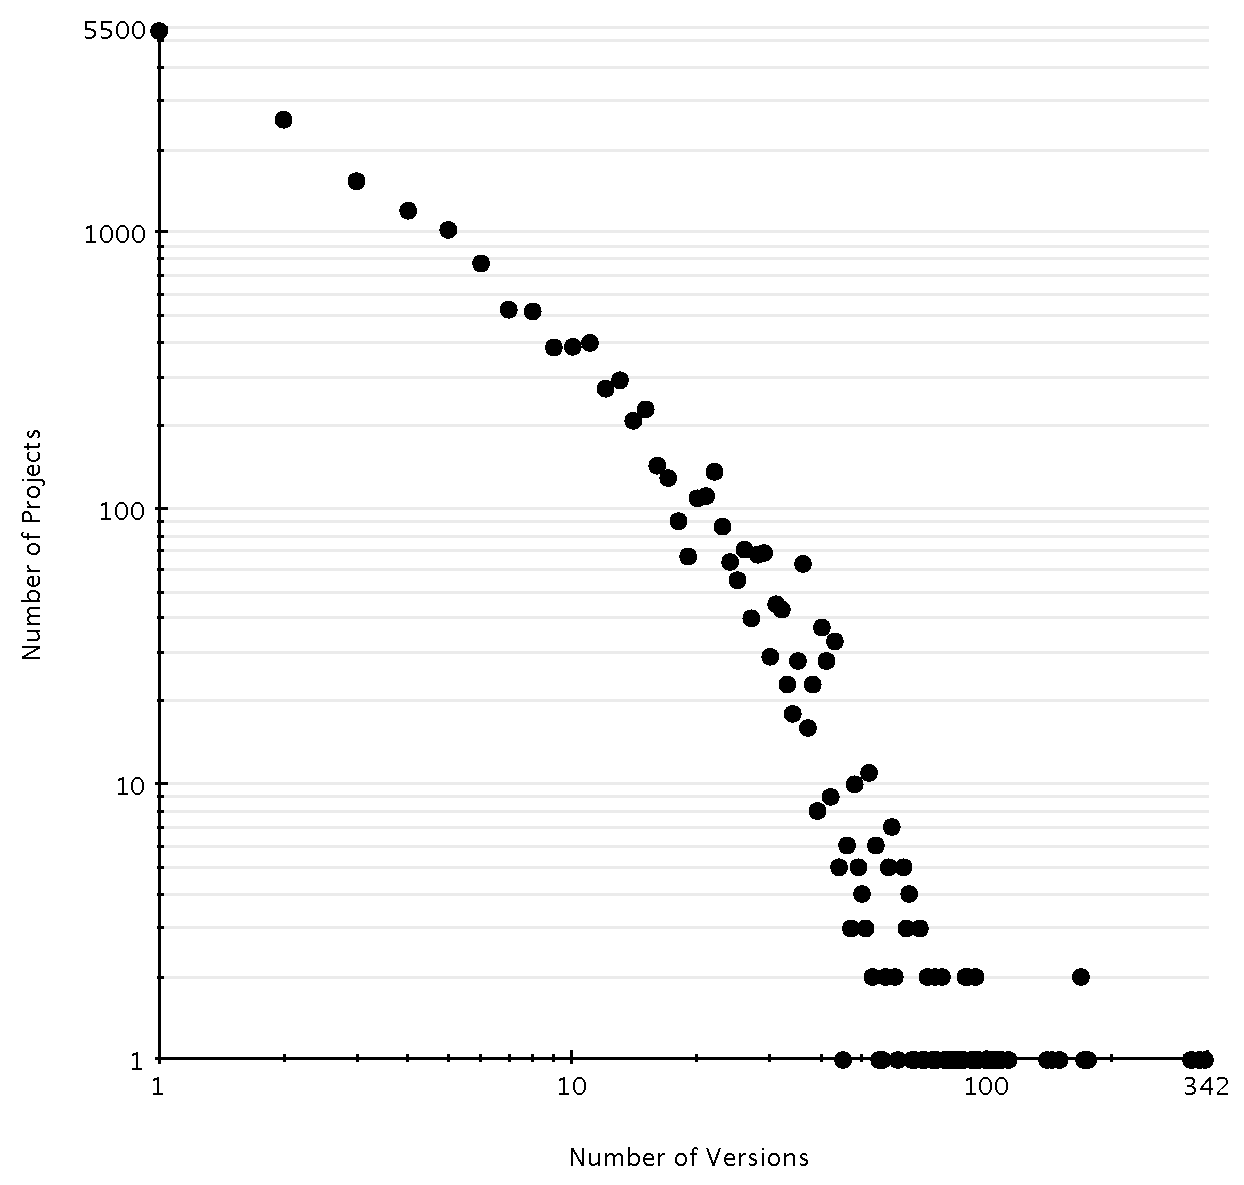
\includegraphics[scale=0.6]{version_count.pdf}
	\caption{Distribution of
Version Count Among Project Population}
	\label{fig:version-count}
\end{figure*}

The statistical mesurements presented in Table~\ref{tbl:repository}
indicate that we have 17,505 projects and the data set's median
is 3, which means that almost 50\% (8,753 projects) of the project
population has 1 to 3 versions.
Note that the Maven repository has many projects with a
few number of versions. For instance, there are numerous projects with a
number of versions that is less than ten.
There are a few projects containing ten
versions and only a few with hundreds of versions. The maximum number of
versions for a project is 337. The 3$^{rd}$ quartile measurement
also indicated that 75\% (13,129) of the projects have a maximum of 8 versions.

\section{Results and Analysis}
\label{sec:res}

\begin{table}
\centering
\caption{Bug Categorisation According to FindBugs}
\label{tbl:bug-cat}
\begin{tabular}{l p{15em}}
\hline
Category & Description\\
\hline
Bad Practice & Violations of recommended and essential
coding practice. \\
Correctness & Involves coding mistakes resulting in code
that was probably not what the developer intended. \\
Experimental & Includes unsatisfied obligations. For instance,
forgetting to close a file. \\
Internationalisation & Indicates the use of non-localized methods. \\
Multi-Threaded Correctness & Thread synchronization issues. \\
Performance & Involves inefficient memory usageallocation, usage 
of non-static classes. \\
Style & Code that is confusing, or
written in a way that leads to errors.\\
Security & Contains two subcategories, namely: {\it Security} and {\it
Malicious Code}. Involves code that could lead to security breach. \\
\hline
\end{tabular}
\end{table}

Our findings can be analyzed at two levels. First, we discuss some
primary observations concerning the security bugs of the Maven repository as a whole.
Then, we provide a comprehensive analysis of the results and highlight our key findings.

\subsection{Overview and Initial Results}
\label{sec:overview}

FindBugs separates software bugs into seven categories (see
Table~\ref{tbl:bug-cat}). Two of them involve security: {\it Security} and {\it
Malicious Code}. From the total number of the artifacts, 4,270 of them contained
at least one bug coming from the first category
and 45,145 coming from the second.

Another observation involves bugs that we could call {\it
severe}. Such bugs are related to vulnerabilities that appear due to the lack of user-input
validation and can lead to damaging attacks like {\sc sql} injection~\cite{RL12} and
Cross-Site Scripting~\cite{WS08}. Note that to exploit such vulnerabilities, a malicious user does
not have to know anything about the applications internals. For all the other
bugs, another program should be written either to incorporate references to
mutable objects, access non-final fields and others. In addition, as
bug descriptions indicate,\footnote{\url{http://findbugs.sourceforge.net/bugDescriptions.html}}
if an application has bugs like these, it might have more vulnerabilities that FindBugs doesn't
report. Table~\ref{tbl:sev} presents the number of {\sc jar}s where at least one of these
bugs exists. In the following section we provide results separately for this
subcategory.

\begin{table*}
\centering
\caption{Number of Versions that Contain at Least One Severe Security Bug}
\label{tbl:sev}
\leavevmode
	\begin{tabular}{l r}
	\hline
	Bug Description & Number of Versions\\
 	\hline
	{\sc hrs}: {\sc http} cookie formed from untrusted input & 149\\
	{\sc hrs}: {\sc http} response splitting vulnerability & 1,564\\
	{\sc pt}: absolute path traversal in servlet  & 92\\
	{\sc pt}: relative path traversal in servlet & 50\\
	{\sc sql}: nonconstant string passed to execute method on an {\sc sql} & 1,817\\
	{\sc sql}: a prepared statement is generated from a nonconstant String & 1,438\\
	{\sc xss}: {\sc jsp} reflected cross site scripting vulnerability & 17\\
	{\sc xss}: Servlet reflected cross site scripting vulnerability in error page & 88\\
	{\sc xss}: Servlet reflected cross site scripting vulnerability & 140\\
	\hline
	\end{tabular}
\end{table*}

Figure~\ref{fig:bug-per} shows how software bugs are distributed among the
repository. Together with the {\it Bad Practice} bugs and the {\it Style} bugs,
security bugs (the sum of the {\it Security} and {\it Malicious Code}
categories) are the most popular in the repository. This could be an indication
that programmers write code that implements the required functionality without considering
its many security aspects. In the following section we
show the correlation of security bugs with all the other categories. An interesting observation is
that 5,601 (31.99\%) projects, containing 32,689 artifacts (28.57\%), did not
have any bugs at all. These cases involved small artifacts with a minimum number of classes.
This goes along with the relationship between the size of an artifact and it's
bugs that is presented in the upcoming section.

\begin{figure*}
	\centering
	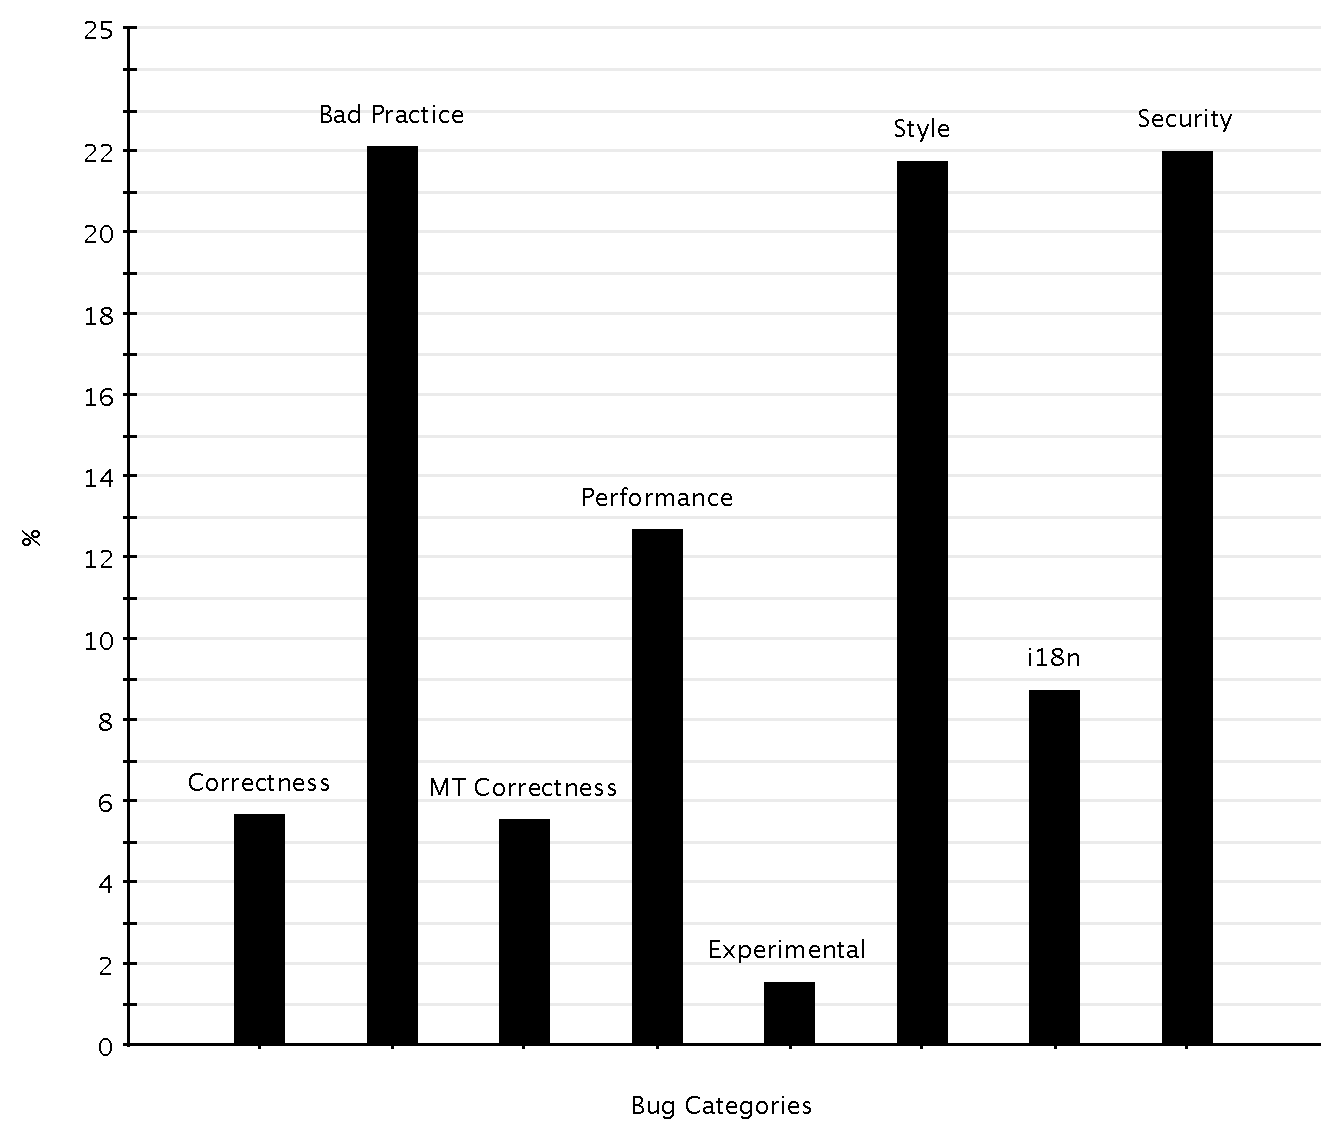
\includegraphics[scale=0.6]{bug_percent}
	\caption{Bug Percentage in Maven Repository}
	\label{fig:bug-per} 
\end{figure*}

As we mentioned earlier, during the experiment we managed to retrieve the
dependencies of every version. Based on this information we created a graph
that represented the snapshot of the repository that we were analyzing. The
nodes of the graph represented the versions and the vertices their dependencies.
We have to mention here that the graph is not representative. For instance, if
a dependency was pointing only to a project (and not to a specific version), we chose to
select the latest version found on the repository. Also, this graph is not
complete. This is because threre were missing versions.
Practically, the corresponding {\it pom}, or {\it war} files existed on the
repository, but the {\sc jar} file did not. From the 56,5680 vertices, 191,433
belonged to the first category while 16,4234 belonged to the second. Finally,
the graph contained 80,354 nodes. Obviously the number does not correspond to
the number of the total versions (see Section~\ref{sec:data}). This is because
some versions did not contain any information about their dependencies so they
are not represented in the graph. After creating the graph, we ran the PageRank
algorithm~\cite{BP98} on it and retrieved all PageRanks for every node. Then we
examined the security bugs of the 50 most popular nodes based on their PageRank.
33 of them contained security bugs while two of them contained severe bugs.
Finally, 25 of them were latest versions at the time.

\subsection{Analysis}
\label{sec:analysis}

\subsubsection{How Security Bugs Evolve Over Time}

\subsubsection{Persistense of Security Bugs}

\subsubsection{The Relation of Defects with the size of an Artifact}

\subsubsection{Security Bugs {\sc vs} Other Bug Categories}

\section{Discussion}
\label{sec:dis}

\section{Related Work}
\label{sec:rel}

There are numerous methods for mining software repositories in the context
of software evolution~\cite{KCM07}. In this section we focus on the ones
that highlight the relationship between software bugs and evolution and try to
extract useful conclusions. The key idea behind this concept is
similar to ours: the combination of information like bug decriptions,
documentation and others with the information retrieved from either the source
or object code of a project version.

{\it Refactoring identification} through software evolution is an approach used to
relate refactorings with software bugs. Wei{\ss}gerber et al. found that a high
ratio of refactorings is usually followed by an increasing ratio of bug
reports~\cite{WD06}. In addition, they indicated that software bugs are sometimes introduced
after an incomplete refactoring~\cite{GW05}.
Ratzinger et al.~\cite{RSG08} showed that the number of bugs decreases, when the number of
refactorings increases. Finally, Kim M. et al.~\cite{KCK11} indicated that {\sc api}-level
refactorings aid bug fixes.

Using {\it micro patterns} is a method proposed by Kim et al.~\cite{KPW06}
to detect bug-prone patterns among source code. Micro patterns describe programming
idioms like inheritance, data management, immutability and others. The approach involved
the examination of all revisions of three open-source projects to extract bug
introduction rates for each pattern. Gil et al.~\cite{GM05} analyzed the
prevalence of micro patterns across five Sun {\sc jdk} versions to conclude that
pattern prevalence tends to be the same in software collections.

{\it Querying techniques} are used to answer a broad range of questions
regarding the evolution history of a project~\cite{HG05}. Bhattacharya et
al.~\cite{BN11, B11} proposed a framework that is based upon
recursively enumerable languages. The framework can correlate software
bugs with developers in various ways. For instanse, return the list of
bugs fixed by a specific developer. Fischer et al.~\cite{FPG03} proposed
an approach for populating a release history database that combines code
information with bug tracking data. In this way, a developer can couple files
that contain common bugs, estimate code maturity with respect to the bugs
and others. The ``Ultimate Debian Database''~\cite{NZ10} is an {\sc sql}-based
framework that integrates information about the Debian project from various
sources to answer queries related to software bugs and source code.

D'Ambros et al. have used {\it bug history analysis} to detect
the critical components of a project~\cite{D08}. This is done by using an
evolutionary meta-model~\cite{DL08}. The same approach was
also used by Zimmermann et al.~\cite{ZNA08} to check the correlation
of bugs with software properties like code complexity, process quality and others
and predict future properties.

Contrary to the above, our work focuses on the subset of security bugs.
Focusing on such bugs is not a new idea. Massacci et al.~\cite{MNN11} observed
the evolution of software defects by examining six major versions of Firefox.
To achieve this they created a database schema that contained information
coming from the ``Mozilla Firefox-related Security Advisories'' ({\sc mfsa})
list,~\footnote{\url{http://www.mozilla.org/projects/security/known-vulnerabilities.html}}
Bugzilla entries and others. Their findings indicated that security bugs are
persistent over time. They also showed that there are many web users that use
old versions of Firefox, meaning that old attacks will continue to work.
Zaman et al.~\cite{ZAH11} focused again on Firefox to study the relation of
security bugs with performance bugs. This was also done by analyzing the project's
Bugzilla. Their research showed that security bugs require more experienced developers
to be fixed. In addittion, they suggested that security bug fixes are more complex than the
fixes of performance and other bugs.
Shahzad et al.~\cite{SSL12} analyzed large sets of vulnerability data-sets to observe
various features of the vulnerabilities that they considered critical. Such features
were the functionality and the criticality of the defects. Their analysis
included the observation of vulnerability disclosures, the behavior of
hackers in releasing exploits for vulnerabilities, patching and others. In
their findings they highlighted the most exploited defects and showed that
the percentage of remotely exploitable vulnerabilities has gradually increased
over the years.

\section{Conclusions and Future Work}
\label{sec:con}

Our work could (?) aid bug-prediction models in the same way as~\cite{BN11}.

\section*{Acknowledgments}

The project is being co-financed by the European Regional Development Fund (ERDF)
and national funds and is a part of the Operational Programme ``Competitiveness \&
Entrepreneurship" (OPCE II), Measure ``COOPERATION" (Action I).

\bibliographystyle{IEEEtran}
\bibliography{msr} 

\end{document}


